% Provenance (never printed): the choice strand of ../economics_series.md (grade 7). Brief: sources/book1/BRIEFS.md,
% g7-01. Chart data: figdata/grade-7/01-scarcity-and-opportunity-cost (PWT 11.0 avh, rgdpe, pop; BLS Consumer
% Expenditure Surveys 2025). Ledger: g7:arkes-blumer-1985.
\chapter{Scarcity and Opportunity Cost}\label{ch:g7:scarcity-and-opportunity-cost}

\begin{openingchart}{Hours worked per worker in a year and income per person, in
2023, one dot per country; income on a times-ten scale.}{Penn World Table 11.0,
average annual hours worked (avh), and real GDP at current purchasing-power
parities (rgdpe) divided by population}
\begin{tikzpicture}
\begin{semilogxaxis}[omincomex, xmin=700, xmax=200000, ymin=1200, ymax=2800,
  xtickten={-3,...,9}, xlabel={Income per person (dollars of 2021, times-ten scale)},
  ylabel={Hours worked per worker in the year}]
\addplot table[x=income, y=hours]
  {figdata/grade-7/01-scarcity-and-opportunity-cost/out/hours_income.csv};
\end{semilogxaxis}
\end{tikzpicture}
\end{openingchart}

% figdata: hours_pairs (DEU 59854 1335; NLD 68499 1439; NOR 89075 1412; IND 8723 2383; BGD 7888 2383; KHM 5527 2389;
% USA 74654 1789; KOR 52389 1910)
% figdata: facts (countries 130, third_size 43, hours_poorest_third_median 2114, hours_richest_third_median 1701)
Every dot is a country. On the right are the richer countries, and most of them
are low on the chart: their workers work fewer hours in a year. A worker in
Germany worked $1\,335$ hours in 2023, one in Norway $1\,412$, where \omterm{def:g6:living-standards:income-per-person}{income per person}
was $89\,075$ dollars; a worker in India or Bangladesh worked $2\,383$ hours, about a
thousand hours more, and \omterm{def:g6:living-standards:income-per-person}{income per person} in India was $8\,723$ dollars. Among the 43 poorest
of the 130 countries, the middle value is $2\,114$ hours; among the 43 richest,
$1\,701$ hours. The dots are scattered: the United States ($1\,789$ hours) and Korea
($1\,910$ hours) are rich and work long hours.

Why would richer people choose to work less? Each person has 24 hours a day, rich
or poor. An hour spent at work is an hour not spent resting, with one's family or
at a game. This chapter is about that kind of choice: when you cannot have
everything, getting one thing means giving up another. It will find two forces at
work when a wage rises, and they pull in opposite directions.

\begin{recall}
Hours worked per worker were measured in \cref{ch:g6:school-and-work}, \omterm{def:g6:living-standards:income-per-person}{income per
person} in \cref{ch:g6:living-standards}, and the \omterm{def:g6:reading-economic-charts:times-ten-scale}{times-ten scale} in
\cref{ch:g6:reading-economic-charts}.
\end{recall}

\begin{omfigure}
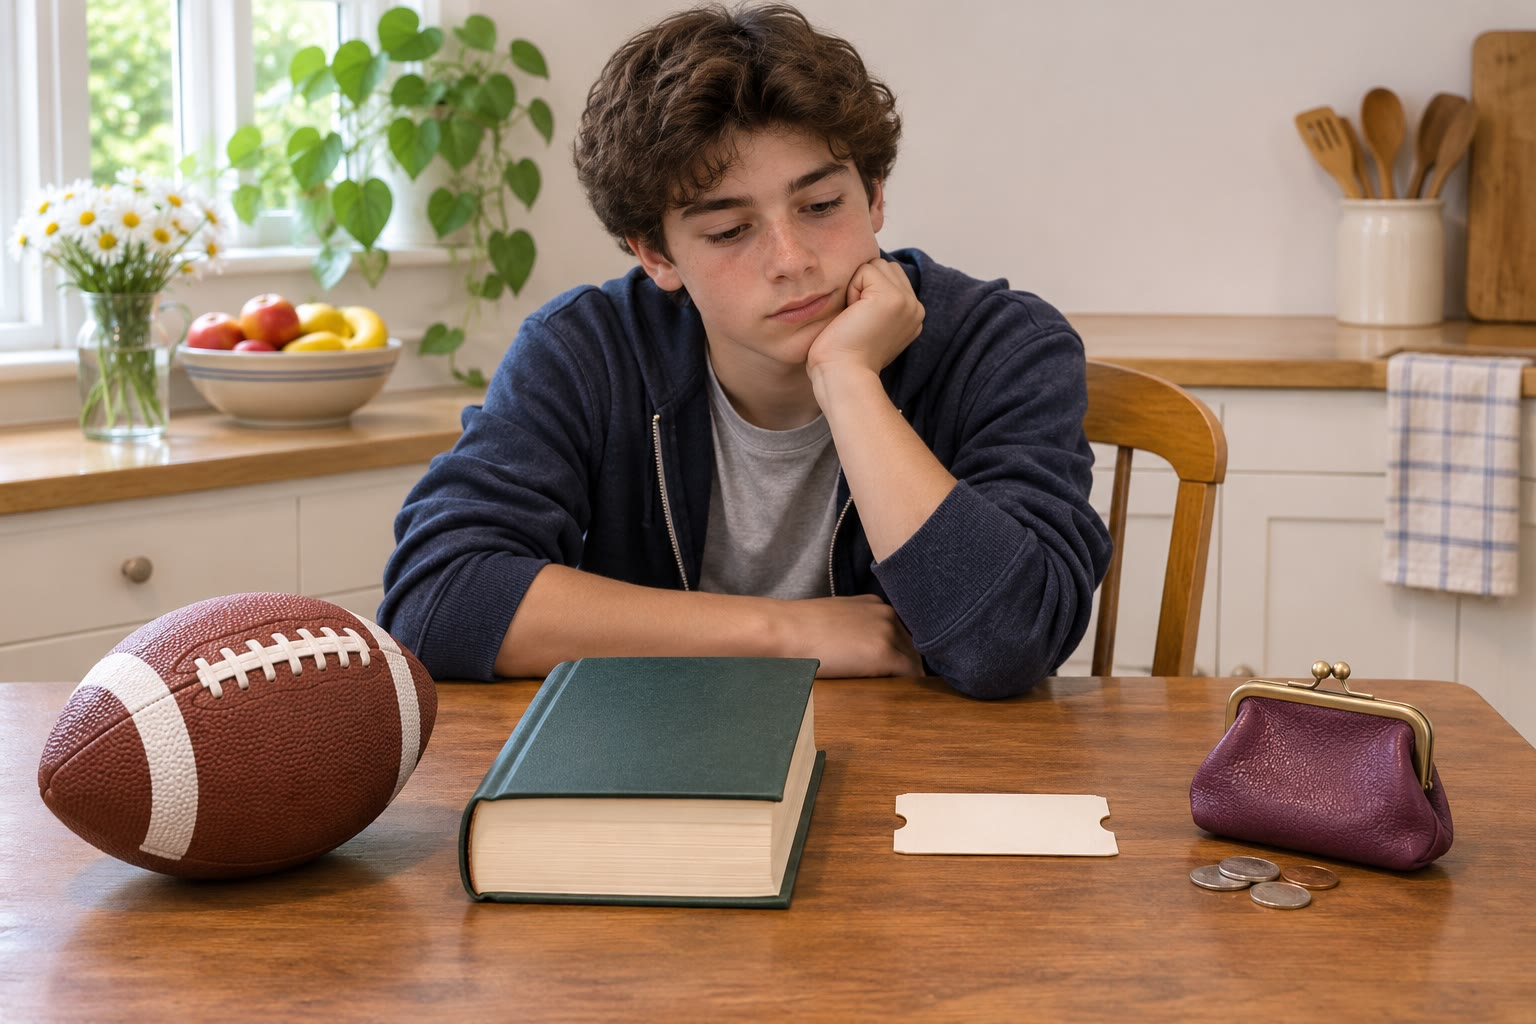
\includegraphics[width=0.55\linewidth]{images/book1/ai/g7-scarcity-and-opportunity-cost-choice.jpg}

{\small A ball, a book or a cinema ticket, and money for only one of them. Choosing
one means giving up the others.}
\end{omfigure}

\section{Wants and means}

People want more things than they can have: more food of a better kind, a bigger
home, more trips, more time with friends, more sleep. The means to get them ---
money, time, land, workers, machines --- are limited.

\begin{definition}[Scarcity]\label{def:g7:scarcity-and-opportunity-cost:scarcity}
\emph{Scarcity}\index{scarcity} is the situation in which people's wants are larger
than the means to satisfy them, so that they must choose which wants to satisfy
and which to leave.
\end{definition}

\omterm{def:g7:scarcity-and-opportunity-cost:scarcity}{Scarcity} does not mean that a thing is rare. Bread is not rare, but a family with
a budget of 2\,000 dalens a month cannot buy unlimited bread \emph{and} everything
else. Even a very rich person faces \omterm{def:g7:scarcity-and-opportunity-cost:scarcity}{scarcity}: he or she has only 24 hours a day.

\begin{omfigure}
\begin{tikzpicture}[econ, x=0.55cm, y=1cm]
  % an invented school day: sleep 9, school 7, travel 1, homework 1.5, meals 1.5, free 4
  \def\seg#1#2#3#4{\fill[#3] (#1,0) rectangle (#2,0.8); \draw (#1,0) rectangle (#2,0.8);
    \node[font=\scriptsize, align=center] at ({(#1+#2)/2},0.4) {#4};}
  \seg{0}{9}{omMeth!25}{sleep\\9 h}
  \seg{9}{16}{omDef!30}{school\\7 h}
  \seg{16}{17}{black!12}{}
  \seg{17}{18.5}{omProp!35}{}
  \seg{18.5}{20}{black!28}{}
  \seg{20}{24}{omThm!25}{free\\4 h}
  \node[font=\scriptsize] (tr) at (13.6,1.45) {travel 1 h};
  \node[font=\scriptsize] (hw) at (17.75,1.45) {homework 1.5 h};
  \node[font=\scriptsize] (ml) at (21.9,1.45) {meals 1.5 h};
  \draw (tr.south east) -- (16.5,0.8);
  \draw (hw.south) -- (17.75,0.8);
  \draw (ml.south west) -- (19.25,0.8);
  \foreach \h in {0,6,12,18,24} \node[font=\scriptsize, below] at (\h,0) {\h};
  \node[font=\scriptsize, below] at (12,-0.35) {hours};
\end{tikzpicture}

{\small The 24 hours of an invented school day. Every extra hour for one activity
must be taken from another.}
\end{omfigure}

\section{To choose is to give up}

\begin{definition}[Choice set]\label{def:g7:scarcity-and-opportunity-cost:choice-set}
A person's \emph{choice set}\index{choice set} is the list of all the options that
he or she can afford, with the money and the time available.
\end{definition}

An option outside the \omterm{def:g7:scarcity-and-opportunity-cost:choice-set}{choice set} is not a choice at all: a trip that costs 500
dalens is not in the \omterm{def:g7:scarcity-and-opportunity-cost:choice-set}{choice set} of someone who has 60 dalens. Inside the \omterm{def:g7:scarcity-and-opportunity-cost:choice-set}{choice set},
choosing one option means giving up all the others.

\begin{omfigure}
\begin{tikzpicture}[econ, x=1cm, y=1cm,
  opt/.style={draw, rounded corners=2pt, fill=omMeth!12, align=center, font=\scriptsize,
    minimum width=3.2cm, minimum height=1cm}]
  \node[draw, rounded corners=2pt, fill=omDef!20, font=\footnotesize, align=center]
    (s) at (0,0) {Saturday afternoon\\40 dalens, 4 hours};
  \node[opt] (a) at (-4.2,-2) {football with friends\\costs 0 dalens\\worth 30 dalens to Lina};
  \node[opt] (b) at (0,-2) {cinema\\costs 12 dalens\\worth 45 dalens to Lina};
  \node[opt] (c) at (4.2,-2) {help at a market stall\\earns 30 dalens\\no pleasure, no pain};
  \draw[-{Stealth}] (s) -- (a); \draw[-{Stealth}] (s) -- (b); \draw[-{Stealth}] (s) -- (c);
\end{tikzpicture}

{\small Lina's \omterm{def:g7:scarcity-and-opportunity-cost:choice-set}{choice set} for a Saturday afternoon (invented). Each option takes the
whole afternoon; she can take only one.}
\end{omfigure}

\section{Opportunity cost}

\begin{definition}[Opportunity cost]\label{def:g7:scarcity-and-opportunity-cost:opportunity-cost}
The \emph{opportunity cost}\index{opportunity cost} of a choice is the value of the
best option given up to make it.
\end{definition}

Only the \emph{best} option given up counts, not all of them: Lina cannot go to
the football game and work at the stall in the same afternoon, so she gives up only
one of them by going to the cinema.

\begin{example}
For Lina, the cinema is worth 45 dalens of pleasure, minus the 12 dalens of the
ticket: a net value of 33 dalens. Football is worth 30 dalens and costs nothing:
30 dalens. Working at the stall brings 30 dalens of pay. The best alternative to
the cinema is worth 30 dalens (football or the stall, which tie), so the \omterm{def:g7:scarcity-and-opportunity-cost:opportunity-cost}{opportunity
cost} of the cinema is 30 dalens. The cinema's net value, 33 dalens, is larger: it
is the best choice. If the stall paid 40 dalens, the \omterm{def:g7:scarcity-and-opportunity-cost:opportunity-cost}{opportunity cost} of the
cinema would be 40 dalens, and working would be the best choice.
\end{example}

\begin{measure}[Valuing time]
Money is easy to count; time is harder. A first estimate of what an hour is worth to
a person is what that person could earn in an hour of extra work: the hourly wage.
It is only a first estimate. Many people cannot choose to work one more hour, and an
hour of rest after ten hours of work is worth more than the first hour of a free
day.
\end{measure}

The \omterm{def:g7:scarcity-and-opportunity-cost:opportunity-cost}{opportunity cost} of an hour rises when the hourly wage rises. This simple idea
is a model of how people choose. Applied to free time, it gives a surprise: when the
wage rises, an hour of rest costs more, so by this force alone people would rest
less and work more. A second force pulls the other way. A higher wage also makes a
person richer, and richer people want more of most things, rest included. This
pull of a larger income is called the \emph{income effect}\index{income effect}.
The model alone does not say which of the two forces wins.

\begin{model}{Choosing by opportunity cost}
\assumes A person compares the options in the \omterm{def:g7:scarcity-and-opportunity-cost:choice-set}{choice set} and picks the one whose
value is larger than the value of the best option given up.
\predicts When the hourly wage rises, the \omterm{def:g7:scarcity-and-opportunity-cost:opportunity-cost}{opportunity cost} of time rises: people
buy more goods and services that save time, such as meals prepared by others. For
free time the model gives no sign by itself: a dearer hour of rest pushes towards
more work, a larger income towards more rest.
\tested Richer households spend a larger share of their food budget on meals
prepared by others (the chart below). The hours of the opening chart, and the long
fall of hours as wages rose since 1950 (\cref{ch:g6:school-and-work}), are
consistent with the income effect having won so far; they do not test the
\omterm{def:g7:scarcity-and-opportunity-cost:opportunity-cost}{opportunity cost} alone, because both forces act at once.
\breaks Habits and rules: many workers cannot choose their hours. People also let
costs they have already paid steer their choices (the section ``A cost already
paid'').
\end{model}

\begin{omchart}{Spending on food away from home (restaurants, canteens, take-away
meals) as a share of all spending on food, in the United States in 2025, for five
groups of households ranked by income, each one fifth of all
households.}{U.S. Bureau of Labor Statistics, Consumer Expenditure Surveys, 2025,
table 1101 (quintiles of income before taxes); food away from home divided by
food}
\begin{tikzpicture}
\begin{axis}[omrecord, ybar, bar width=22pt, ymin=0, ymax=50, grid=none, ymajorgrids,
  enlarge x limits=0.15, xtick=data,
  xticklabels={Lowest fifth, Second, Third, Fourth, Highest fifth},
  x tick label style={font=\footnotesize}, ylabel={Percent of food spending},
  nodes near coords={\pgfmathprintnumber[fixed, fixed zerofill, precision=1]{\pgfplotspointmeta}},
  every node near coord/.append style={font=\scriptsize},
  height=0.45\linewidth]
\addplot[fill=omMeth!55, draw=omMeth] table[x=quintile, y=away_share]
  {figdata/grade-7/01-scarcity-and-opportunity-cost/out/meals_away.csv};
\end{axis}
\end{tikzpicture}
\end{omchart}

% figdata: meals_away (1: 5156, 1556, 30.2; 5: 18415, 8108, 44.0)
The households of the lowest fifth spent $1\,556$ of their $5\,156$ food dollars on
meals away from home: $30.2\,\%$. The highest fifth spent $8\,108$ of $18\,415$
dollars: $44.0\,\%$. This fits the model: a meal cooked by someone else saves an
hour of cooking, and an hour is worth more to a person who earns more. It is not a
proof. Eating out is also a pleasure, and richer households may simply buy more of
every pleasure.

\section{A cost already paid}

\begin{definition}[Sunk cost]\label{def:g7:scarcity-and-opportunity-cost:sunk-cost}
A \emph{sunk cost}\index{sunk cost} is a cost that has already been paid and cannot
be recovered, whatever one chooses now.
\end{definition}

A \omterm{def:g7:scarcity-and-opportunity-cost:sunk-cost}{sunk cost} is not an \omterm{def:g7:scarcity-and-opportunity-cost:opportunity-cost}{opportunity cost} of any choice that remains, because no choice
can bring it back. The model says to leave it out: compare only what each option
still brings and still costs.

\begin{example}
Tom paid 20 dalens for a concert ticket that cannot be sold or refunded. On the
evening of the concert, he feels ill, and staying home is worth 15 dalens to him,
while the concert, ill as he is, is worth 10. The 20 dalens are gone either way:
they are a \omterm{def:g7:scarcity-and-opportunity-cost:sunk-cost}{sunk cost}. Staying home (15) beats the concert (10). ``I paid for it, so
I must go'' adds the 20 dalens to one side only, and leads to the worse choice.
\end{example}

% ledger: g7:arkes-blumer-1985 (first 60 buyers; first five plays 4.11 / 3.32 / 3.29 tickets; last five, no
% significant difference)
Do people leave \omterm{def:g7:scarcity-and-opportunity-cost:sunk-cost}{sunk costs} out? An experiment in a university theatre tested it.
Among the first 60 people who bought a season ticket, some paid the full price of
15 dollars and the others, chosen at random, were given a discount of 2 or of 7
dollars. Over the first five plays of the season, those who had paid the full price
used more tickets, $4.11$ each on average, than those given a discount, $3.32$ and
$3.29$. Over the last five plays the gap disappeared (Arkes and Blumer, 1985). By the
model, the price already paid should not matter for the decision to go out on a
given evening. Here it did, for a while: this is a place where the model breaks.

\section{Persons, firms and countries}

The same reasoning works for a firm. A baker who owns her shop pays no rent. Using
the shop is not free all the same: she could rent it to someone else. The rent she
gives up is the \omterm{def:g7:scarcity-and-opportunity-cost:opportunity-cost}{opportunity cost} of using it herself.

It works for a country too. A hectare of land near a growing town can grow wheat or
hold houses. The \omterm{def:g7:scarcity-and-opportunity-cost:opportunity-cost}{opportunity cost} of the houses is the wheat no longer grown there,
and the \omterm{def:g7:scarcity-and-opportunity-cost:opportunity-cost}{opportunity cost} of the wheat is the houses not built. Workers, machines and
money spent on one thing are not available for another.

\section{Exercises}

\begin{exercise}[$\star$]\label{exo:g7:scarcity-and-opportunity-cost:1}
Use the values in the text. How many hours did a worker work in 2023 in Germany, and
in India? What is the difference?
\end{exercise}

\begin{exercise}[$\star$]\label{exo:g7:scarcity-and-opportunity-cost:2}
Sami has a free evening. Here is what each option is worth to him, after its
costs: a film at home 8 dalens, a game with friends 14 dalens, reading 11 dalens. He
chooses the game. What is the \omterm{def:g7:scarcity-and-opportunity-cost:opportunity-cost}{opportunity cost} of his choice?
\end{exercise}

\begin{exercise}[$\star$]\label{exo:g7:scarcity-and-opportunity-cost:3}
To visit her aunt, Rosa can take the train (18 dalens, 2 hours) or the bus (10 dalens,
4 hours). (a) What does the train cost more in money? (b) How much time does it save?
(c) If an hour of Rosa's time is worth 3 dalens to her, which trip costs her less in
all?
\end{exercise}

\begin{exercise}[$\star$]\label{exo:g7:scarcity-and-opportunity-cost:4}
A firm can use a free hall for a fair worth 500 dalens, a concert worth 800 dalens, or
a market worth 650 dalens. It chooses the concert. What is the best alternative given
up, and the \omterm{def:g7:scarcity-and-opportunity-cost:opportunity-cost}{opportunity cost}?
\end{exercise}

\begin{exercise}[$\star\star$]\label{exo:g7:scarcity-and-opportunity-cost:5}
Ana paid 25 dalens, which cannot be refunded, for a concert on Friday. On Friday, a
friend invites her to a party worth 30 dalens to her; the concert is now worth 20
dalens to her. (a) Which costs are sunk? (b) Which option does the model predict she
chooses? (c) What would she choose if she counted the 25 dalens as part of the
concert's value?
\end{exercise}

\begin{exercise}[$\star\star$]\label{exo:g7:scarcity-and-opportunity-cost:6}
A firm owns a warehouse it uses for its own goods. Another firm offers to rent it for
1\,200 dalens a month. (a) What is the \omterm{def:g7:scarcity-and-opportunity-cost:opportunity-cost}{opportunity cost}, per month, of using the
warehouse itself? (b) The firm could store its goods elsewhere for 900 dalens a month.
What does the model predict it does?
\end{exercise}

\begin{exercise}[$\star\star$]\label{exo:g7:scarcity-and-opportunity-cost:7}
Cooking dinner takes Ben one hour and costs 6 dalens of food; a ready meal costs 14
dalens and takes no time. (a) If an hour of Ben's time is worth 5 dalens, which is
cheaper for him in all? (b) Ben's wage rises, and an hour is now worth 12 dalens. Which
is cheaper now? (c) What does the model predict about people's purchases of ready
meals when wages rise?
\end{exercise}

\begin{exercise}[$\star\star$]\label{exo:g7:scarcity-and-opportunity-cost:8}
Use the values in the text. (a) How many more hours did a worker in India work in 2023
than one in Norway? (b) How many times larger was \omterm{def:g6:living-standards:income-per-person}{income per person} in Norway? Round
to one decimal.
\end{exercise}

\begin{exercise}[$\star\star$]\label{exo:g7:scarcity-and-opportunity-cost:9}
Describe an observation that would contradict the model ``Choosing by \omterm{def:g7:scarcity-and-opportunity-cost:opportunity-cost}{opportunity
cost}'': what would people do that the model says they do not?
\end{exercise}

\begin{exercise}[$\star\star\star$]\label{exo:g7:scarcity-and-opportunity-cost:10}
An invented country has 100 hectares near its capital. A hectare can grow 5 tonnes of
wheat a year or hold 40 homes. (a) If it builds homes on 30 hectares, how much wheat
does it give up each year? (b) What is the \omterm{def:g7:scarcity-and-opportunity-cost:opportunity-cost}{opportunity cost} of one home, in tonnes of
wheat? (c) And of one tonne of wheat, in homes?
\end{exercise}

\begin{exercise}[$\star\star\star$]\label{exo:g7:scarcity-and-opportunity-cost:11}
A museum is free to enter. A visit takes three hours, and the bus costs 4 dalens.
(a) Is the visit free? Explain using \omterm{def:g7:scarcity-and-opportunity-cost:opportunity-cost}{opportunity cost}. (b) For a person whose hour is
worth 6 dalens and who would otherwise rest, give a first estimate of the visit's cost.
\end{exercise}

\begin{exercise}[$\star\star\star$]\label{exo:g7:scarcity-and-opportunity-cost:12}
In the theatre experiment described in the chapter, suppose the result had been the
opposite: those who paid the most went to fewer plays. (a) Would this contradict the
model? (b) What result would have agreed with the model exactly?
\end{exercise}

\section{Problem: A Saturday in Brenmoor}

\begin{problem}[{Weekend problem --- listing the options of a free day in Brenland's
capital, finding the best one and its opportunity cost, and choosing again when
prices change}]
\label{pb:g7:scarcity-and-opportunity-cost:1}
Everything in this problem is invented. Mira lives in Brenmoor, the capital of
Brenland. On Saturday she has 50 dalens and 8 free hours. She values an hour of her
time at 4 dalens. Her options for the day are:
\begin{center}
\begin{tabular}{lrrr}
\toprule
Option & Money paid (dalens) & Hours & Worth to Mira (dalens) \\
\midrule
A: bus to the beach & 12 (bus) & 8 & 70 \\
B: a museum and a café & 15 & 5 & 45 \\
C: work at her uncle's shop & earns 48 & 8 & 0 \\
D: a concert in town & 55 & 4 & 90 \\
\bottomrule
\end{tabular}
\end{center}

\medskip
\noindent\textbf{Part I --- The options.}
\begin{enumerate}
  \item Which option is not in Mira's \omterm{def:g7:scarcity-and-opportunity-cost:choice-set}{choice set}? Why?
  \item For option B, Mira has 3 hours left. If she spends them resting, what are they
        worth to her?
  \item For each option in the \omterm{def:g7:scarcity-and-opportunity-cost:choice-set}{choice set}, compute its net value: what it is worth to
        Mira, plus what it earns, minus what it costs, plus the value of the hours it
        leaves free.
\end{enumerate}

\medskip
\noindent\textbf{Part II --- The best choice.}
\begin{enumerate}[resume]
  \item Which option is the best? What is its \omterm{def:g7:scarcity-and-opportunity-cost:opportunity-cost}{opportunity cost}?
  \item By how many dalens does the best option beat the next best?
  \item Mira's friend says: ``Working at the shop costs you nothing, you are paid!''
        What does the friend leave out?
\end{enumerate}

\medskip
\noindent\textbf{Part III --- A change.} The bus fare to the beach rises from 12 to 30
dalens.
\begin{enumerate}[resume]
  \item Compute the new net value of option A.
  \item What is the best option now, and its \omterm{def:g7:scarcity-and-opportunity-cost:opportunity-cost}{opportunity cost}?
  \item Mira had already bought, on Friday, a non-refundable bus ticket at the old fare
        of 12 dalens. Does that change the comparison? Explain with the word ``sunk''.
  \item Her uncle now offers 75 dalens for the day at the shop. With the bus ticket
        already paid, compute the net values of A and C again.
  \item What does Mira choose, and what is the \omterm{def:g7:scarcity-and-opportunity-cost:opportunity-cost}{opportunity cost} of her choice, in
        dalens?
\end{enumerate}
\end{problem}
